\section{Timed Petri Nets Processor Architecture and Operation}

	The processor executes the state equation solving only a firing of a transition at a time, this
	way can solve all cases of firings, the simple ones (single firings) and the multiple firings,
	performing as a single-firing sequence, as a result, the hardware is simpler.
	
	The resolution of firings is requested by the threads running on the cores through the system bus,
	as emerging requests that system is running. These firing requests are received by the Timed Petri
	processor and stored in the input queue. This queue is FIFO according to each transition, the
	output of this queue is a binary word of size equal to the number of transitions. This word has
	\emph{ones} in the positions corresponding to transitions with firings requested. The order of the
	bit in the word equals the number of transition over which the firing is requested. The bits that
	correspond to the transitions which has no firing request are \emph{zero}.
	
	The output queue has a similar structure, but its function is to communicate to the threads those
	firings that have been resolved.
	
	\begin{figure}[h]
        \centering
        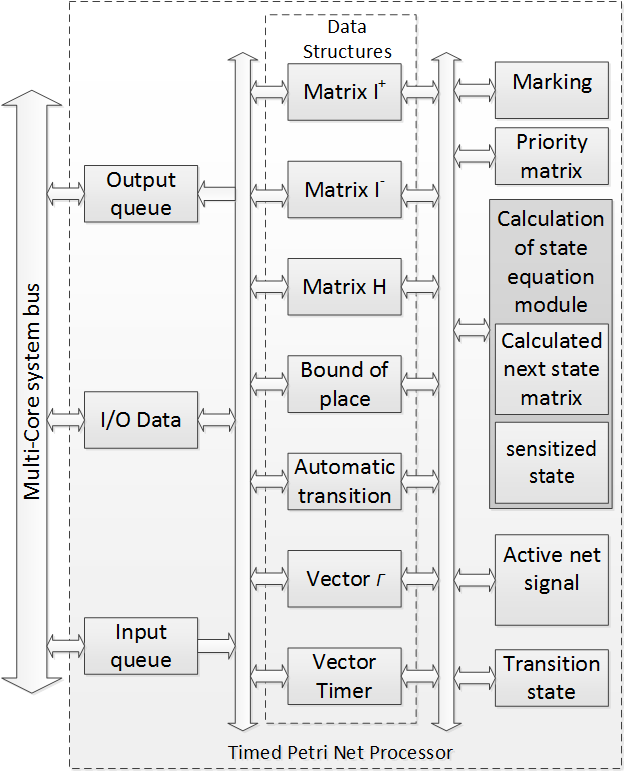
\includegraphics[width=1\linewidth]{./img/timed_petri_nets_processor}
        \caption{Timed Petri Nets Processor}
        \label{fig:time_petri_nets_processor}
    \end{figure}
	
    The data I/O module manages the access of the cores to the matrices and vectors that program the 
    system. The module manages the access of the cores to the matrices and vectors that program the 
    system.
    
    The matrices and vectors described in the equation of state are the system program. This allows 
    us to program the processor directly from the Timed Petri Net.

    Here we have added the inhibitor arcs matrix and the vector indicating the maximum number of tokens 
    in the places. This terms are not present in the state equitions shown in this work but you can 
    consult the work \cite{micolinipereyragalliaalasia} to obtain more information about those elements.

    The module in charge of solving the state equation of the Petri has the following responsabilities:
    La responsabilidad del M�dulo de C�lculo de la Ecuaci�n de estado es la siguiente:
    
    \begin{enumerate}
        \item Calculating the new state that would result from each transition firing only once, thereby 
            generating a number of vectors calculated states equal to the number of transitions. Then, 
            these vectors are stored. This is performed by subtracting the current state parallel to 
            each column of $I^+$ and storing all resulting vectors, which will be evaluated to determine 
            if the new state that each transition would produce is valid. This operation is performed 
            whenever you change the timed Petri Nets Processor status (current marking vector).
        \item Determine which transition is sensitized. To do this, take all vectors calculated in step 
            1 and verify that there is no place to have a negative marking and neither exceeding the
            limit\footnotemark of tokens it can hold.
        \item From the group of sensitized transitions determined at step 2 and its firing has been 
            requested we select the one with higher priority. This transition will be used to determine 
            the new state of the net. This update of the marking vector will be perform by replacing 
            of the current vector with the one calculated in step 1 corresponding to the selected 
            transition. At that moment, in Timer Module, starts the timer corresponding to the
            transition fired.
        \item Compare each component of the $\Gamma$ vector with the one in $Timer$ vector and
        	verify that it meets the following condition:
        	\begin{equation*}
				\Gamma_t \leq Timer_t
			\end{equation*}
        	The fulfillment of this condition means that the transition \emph{t} has reached the
        	delay time required. Then, the transition of higher priority than meets the above condition
        	is chosen to update the marking vector. This means, add to the current marking vector the
        	column of the matrix $I^+$ corresponding to the transition \emph{t}. At the same time the
        	position \emph{t} of the $Timer$ vector is set to zero ($Timer_t = 0$).
        \item Execute the steps 1, 2, 3 and 4 as a continuous cycle.
    \end{enumerate}
    
    The system also has a unit that detects when no transition is sensitized and the $Timer$ vector
    is zero. When this happens, the system generates an interruption notifying that the system has
    finished its execution or is deadlocked. This feature is very useful to verify the operation of
    the design and implementation of the system.
    
    \footnotetext{It is noted that this is a weak bound, since the marks in the squares are incremented 
    in step 4 and the limit is checked in step 2. This simplification facilitates hardware implementation.
    }   



